% Diese Zeile bitte -nicht- aendern.

\documentclass[course=erap]{aspdoc}
\usepackage{amssymb}
\usepackage[utf8]{inputenc}
\usepackage{graphicx}


\graphicspath{{Images/}}

%%%%%%%%%%%%%%%%%%%%%%%%%%%%%%%%%
%% TODO: Ersetzen Sie in den folgenden Zeilen die entsprechenden -Texte-
%% mit den richtigen Werten.
\newcommand{\theGroup}{} % Beispiel: 42
\newcommand{\theNumber}{A215} % Beispiel: A123
\author{Abdalla Mahamid \and Marsel Ivanov Kolovski \and Rafiq Nasrallah}
\date{Sommersemester 2020 } % Beispiel: Wintersemester 2019/20
%%%%%%%%%%%%%%%%%%%%%%%%%%%%%%%%%
% hey, can you see that?  
% 
% Diese Zeile bitte -nicht- aendern.
\title{Gruppe \theGroup{199} -- Abgabe zu Aufgabe \theNumber}
%\footnote{Siehe: https://mathoverflow.net/questions/237132/applications-of-space-filling-curves}
\begin{document}
\maketitle

\section{Einleitung}
\hspace{0.3cm}
In der Mathematik und Informatik ist das Thema „raumfüllende Kurven” sehr bekannt und hat verschiedene Anwendungen. Z.B. es wird in \href{https://mathoverflow.net/questions/237132/applications-of-space-filling-curves}{Google Maps} verwendet, um die Cache-Lokalität einzuführen, dann wenn man sich ein bisschen auf der Karte bewegt, dann will man sich so niedrig wie möglich im Speicher bewegen,der schließlich linear angeordnet ist. Hierzu finden kontinuierliche raumfüllende Kurven eine ihrer Anwendungen.  In diesem Projekt werden wir einen Typ einer der berühmtesten raumfüllenden Kurven untersuchen. Aber was heißt eigentlich “raumfüllende Kurve”?
Raumfüllende Kurven sind ein Verfahren eine zweidimensionale Fläche bzw. Matrix komplett durchzulaufen. Ein historisches Problem ist, dass es nicht möglich war, eine Funktion zu erfinden, die eine Abhängigkeit zwischen eindimensionalen und zweidimenisionalen Flächen findet. Jedoch hat im Jahr 1890 Giuseppe Peano (italienischer Mathematiker)\cite{BaderBook} die Geschichte verändert und eine Lösung dazu gefunden. Später wurde dies Verfahren als Peano-Kurven gennant, wobei eine davon unser Projektthema ist. Obwohl diese Erfindung vor 130 Jahren stattgefunden hat, wird sie heute noch in vielen Gebieten genutzt. Z.B. wird in der Bildverarbeitung (image processing) genutzt. Nehmen wir an, Wir wollen eine Software schreiben, mit der Menschen Bilder mit den Ohren „sehen“ können. Daten werden von einer Kamera (zweidimensional) aufgenommen und auf sinnvolle Weise in einen Ton (eindimensional) umwandeln. Wir müssen dann jedes einzelne Pixel des Bildes einer Zahl zuordnen, die dann eine bestimmte Frequenz hat. Hier stehen die Peano-Meander Kurven zur Verfügung - sie „übersetzen“ die Pixel in eindeutige Zahlen und sind so gut darin, weil die Zahlen zu einem bestimmten Wert konvergieren. D.h. je besser die Auflösung wird, desto leichter kann das Gehirn das gleiche Bild mit einer besseren Qualität anpassen.\cite{scientificamerican}
Das ist nur ein kleines Beispiel einer der vielen Peano-Meander-Kurven-Nutzungsbereich. Im Rahmen dieses Projektes werden wir auf eine konkrete Peano-Meander-Kurve n-tes Grades eingehen, die spezifische zweidimensionale Flächen füllt. Sie hat als Basis ihre Grafik 9 Knoten, und wenn wir sie in einer gewissen Reihenfolge durchlaufen, besuchen wir alle Knoten und zeichnen eine Peano-Meander-Kurve.
In unserer Ausarbeitung zeigen wir einen Algorithmus, der für Eingabe von n (n ist die Grad der Peano-Meander-Kurve) die Abfolge der Knotenpunkte als Koordinaten repräsentiert. Wir werden diesen Algorithmus benutzen, um die richtige Reihenfolge der Koordinaten im Assembler zu bekommen und danach die entsprechende Peano-Meander-Kurve mit C in einer SVG-Datei darzustellen. Letztlich werden wir die Laufzeit unseres Codes nach allen gefundenen Optimierungen analysieren.   

\section{Lösungsansatz}
\hspace{0.3cm}
Unser Ziel ist ein Codegerüst in C zu erarbeiten, welches die Funktionen definiert und aufgerufen werden. Wir erstellen eine Assemblerdatei, die ebenfalls die Knotenpunkte der Peano-Meander-Kurve n-ten Grades erzeugt. Um das zu erreichen, teilen wir die Aufgabe in folgende Unteraufgaben:
\begin{enumerate}
  \item Peano-Meander-Koordinatenpunkte inklusive Anfangspunkte definieren.
  \item Die Struktur der Peano-Meander-Kurve 2-ten bzw. n-ten Grades verstehen.
  \item Eine mathematische Abbildung finden, die jeden Koordinatenpunkt der Peano-Meander-Kurve 1-ten Grades auf die Koordinatenpunkte der Peano-Meander-Kurve 2-ten Grades abbildet.
  \item Eine Bijektion zwischen Zahlen und den Koordinaten der Abfolge der Knotenpunkte der Peano-Meander-Kurve n-ten Grades erschaffen.
  \item Eine Funktion von jedem Koordinatenpunkt der Peano-Meander-Kurve 1-ten Grades auf die Koordinatenpunkte der Peano-Meander-Kurve n-ten Grades erstellen.\newline
\end{enumerate}

\large\textbf{Peano-Meander Koordinatenpunkte definieren}\newline

Da wir in unserer Assemblerfunktion Koordinaten bearbeiten sollen, definieren wir nun, welche Knotenpunkte der Peano-Meander Kurve eigentlich angeschaut werden sollen: jeder Punkt, wobei die Figur eine Kurve darstellt, inklusive den beiden Anfangs- und Ausgangspunkte, bezeichnen wir als Peano-Meander Koordinatenpunkt. Hier kann man sich eine sehr wichtige Frage stellen: welcher Koordinatenpunkt soll der Anfangspunkt der Peano-Meander-Kurve sein?
Da sowohl in der Mathematik, als auch in der Fachliteratur der Anfangspunkt unten links ist\cite{BaderBook}, haben wir uns entschieden von unten links zu fangen. Folglich bezeichnen wir die Ecke unten links mit $(0,0)$. Um unsere Idee möglichst ausführlicher zu erklären, schauen wir uns erstens die Struktur der Peano-Meander Kurve n-ten Grades für $n=2$ bzw. beliebiges $n$ an.\newline

\large\textbf{Struktur der Peano-Meander-Kurve 2-ten Grades}\newline

Wir haben von unseren Beobachtungen und der Fachliteratur die Struktur der Peano-Meander Kurve erstens für $n=2$ und dann für beliebigen Grad $n\in \mathbb {N}$ verstanden. \newline
Sei $A_n$ die Peano-Meander-Kurve $n$-ten Grades. Die Abbildung lässt vermuten, dass $A_2$ sich ganz grob in neun $3\times3$ Quadrate (durch die roten Striche geteilt) teilen lässt. Jedes dieser Quadrate enthält entweder die vorherige Peano-Meander-Kurve ($A_1$), oder eine modifizierte $A_1$ Kurve und ist 

\noindent\begin{minipage}{.65\textwidth}
mit einer zusätzlichen grünen Striche (Abbildung rechts) mit dem nächsten Quadrat verbunden. (Bemerkung: wenn man die grünen Striche verbindet, bekommt man eine Darstellung der $A_1$). Als modifizierte Figur werden wir solche Figuren bezeichnen, die entweder um 90 Grad gedreht wurden oder Spiegelungsabbildungen von einer der beiden Achsen sind (mehr dazu später).\newline
\end{minipage}%
\begin{minipage}
    \centering
    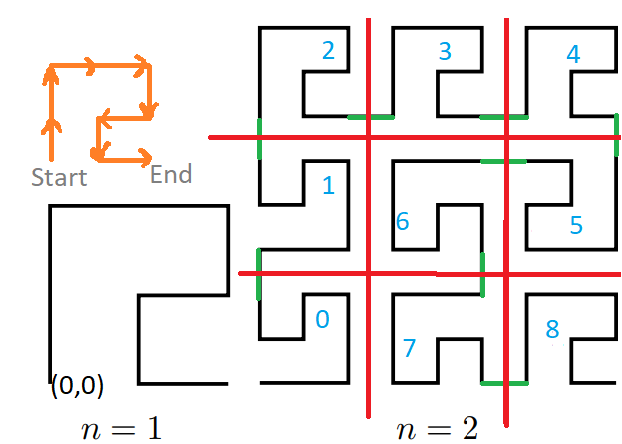
\includegraphics[width=5cm]{ausa.png}
    \caption{}
    \label{fig:ausa.png}
\end{minipage}

\large\textbf{Struktur der Peano-Meander Kurve n-ten Grades}\newline

Schauen wir jetzt, ob dieselbe Abhängigkeit für beliebiges $n$ gilt. Unabhängig von $n$ kann man $A_n$ wieder in neun Quadrate teilen. Worin liegt dann der Unterschied zwischen $A_2$ und $A_n$?
 Jedes dieser Quadrate ist im Vergleich zu $A_2$ anstatt $A_n$ entweder $A_{n-1}$, oder eine modifizierte $A_{n-1}$ Kurve und ist wieder mit einem zusätzlichen Strich mit dem nächsten Quadrat verbunden, um alles in eine einzelne Zusammenhangskomponente zu bringen. Daraus folgt, dass im Allgemeinen für die Anzahl der Koordinatenpunkte gilt: $|A_n| = 9 \cdot  |A_{n_-_1}|$ und $|A_1|=9$, wobei $|A_n|$ die Anzahl der Peano-Meander Koordiantenpunkte in $A_n$ ist. Aus dieser Rekursionsgleichung kann man schließen, dass die Anzahl der Peano-Meander Koordiantenpunkte für ein beliebiges $n$ $|A_n| = 9^n$ ist.
Was man noch sehen kann, ist, dass die Konstruktion der Peano-Meander-Kurve immer eindeutig ist. Das heißt, dass diese neun Quadraten in eine strenge Korrelation miteinander stehen. Folglich gibt es keine Randomisierung bei dem Aufbau von $A_n$. Um diese Korrelation genauer zu begründen schauen schauen wir uns im Folgenden die Konstruktion von $A_2$ an. \newline%({\footnotesize{Für die Nummerierung der Quadraten sieh Abbildung} \ref{fig:ausa.png}}) 

\large\textbf{Quadrat 0}: Wie bereits erwähnt, ist unser Anfangspunkt unten links, also ist unser erst zu beschreibendes Quadrat, dieses das in der Ecke unten links liegt. Dieses Quadrat ist aber keine direkte Abbildung von der vorherigen Peano-Meander-Kurve ($A_1$), sondern eine modifizierte Variante von $A_1$. Was wir erstens bemerkten, dass wenn $A_1$ nun um $90$ Grad gegen den Uhrzeigersinn gedreht und über die x-Achse für $x=1$ gespiegelt wurde, das gesuchte Quadrat erzeugt kann. Dieses Verfahren ist aber nicht das, wonach wir streben. Wir wollen einen iterativen Algorithmus implementieren. Das heißt, wir möchten nicht mit Quadraten umgehen, sondern mit ihren Koordinatenpunkten arbeiten. Folglich sollten wir eine Funktion erzeugen, die jeden Peano-Meander Koordiantenpunkte von $A_1$ im Quadrat $0$ in $A_2$ abbildet. Mit der Zeit hatten wir gesehen, dass anstatt dieser Rotierungen es ausreicht, jedem Peano-Meander Koordinatenpunkt von $A_1$ seiner Y-Koordinate mit seiner X-Koordinate umzutauschen. \newline \textbf{Mathematische Formel:} $\{(y,x) | (x,y) \in A_1\}$.\newline


\large\textbf{Quadrat 1}: Intuitiv kann man sehen, dass das nächste Quadrat links zentral liegen sollte, da wir von unten links angefangen haben. Dieses Quadrat ist identisch zu Quadrat $0$. Der Unterschied liegt darin, dass die Koordinaten mit einem Offset: $(x,y) \to (x,y+3)$ versetzt werden muss.\newline


\large\textbf{Quadrat 2}: Dieses Quadrat ist offensichtlich identisch zu der vorherigen Kurve ($A_1$). Wie Quadrat 1 fehlt nur den Offset der Koordiantenpunkte. Dieses Quadrat liegt oben links. Folglich ist der Offset: $(x,y) \to (x,y+6)$.   \newline

\large\textbf{Quadrat 3}: Wie Quadrat 2 ist wieder $A_1$, aber mit verschiedenem Offset. Da es sich oben in der Mitte befindet, ist der resultierende Offset der Folgende:: $(x,y) \to (x+3,y+6)$.\newline

\large\textbf{Quadrat 4}: Wie die vorherigen zwei Quadrate ist hier nun der Offset verschieden: $(x,y) \to (x+6,y+6)$.\newline

\large\textbf{Quadrat 5}: Dieses Quadrat ist die modifizierte $A_1$. Erstens, was wir bemerkten, dass dieses Quadrat um 180 Grad rotiert wurde. Aber, wie bei Quadrat $0$ schon gesagt, reicht uns nur das nicht, weil wir uns für die Koordinatenpunkte interessieren. Nach vielen Überlegungen sahen wir, dass wenn jeder Koordinatenpunkt von $A_1$ von $(x,y)$ auf $(2-x,2-y)$ abgebildet wird, man genau die gesuchte gespiegelte Modifikation von $A_1$ bekommt. Nun stellt sich die Frage woher die Verschieben um 2 kommt. Unsere Quadrate in $A_2$ sind $3\times3$, das heißt,  die niedrigste und höchste Koordinaten eine Differenz von $2$ haben, anders gesagt werden immer “symmetrische Knotenpunkte” über dem Hauptdiagonale umgetauscht.  Für $A_n$ würde analog $(x,y)\to(3^{n-1}-1-x,3^{n-1}-1-y)$, da die Länge der Achsen von $A_n$,wie schon erwähnt, gleich $3^n$ ist. Nur das mit sich reicht natürlich nicht, weil diese Funktion $A_1$ nur umgedreht hat. Wir möchten die Koordiantenpunkte dieses Quadrat an der richtigen Stelle positionieren und dazu benutzen wir wieder Offsets wie folgt:  Offset: $(x,y) \to (x+6,y+3)$.\newline


\large\textbf{Quadrat 6}: Dieses Quadrat wäre sehr schwer abzubilden, wenn Quadraten $0$ und Quadraten $5$ nicht gemacht werden. Dieses Quadrat ist genauso wie Quadrat 0, jedoch ist nach $180$ Grad gedreht und dann wird eine gespiegelte Modifikation von Quadrat 0 gebildet. Hängen wir die beiden Funktionen zusammen, bekommen wir das gesuchte Quadrat.\textbf{Formal:} Seien $f,g : (x,y) \to (x,y)$, $(x,y)\in{A_1}$, wobei $f(x,y) = (y,x)$ und $g(x,y) = (2-x,2-y)$, dann ist $g(f(x))$ die Abbildung jedes Punkt aus $A_1$ im Quadrat 6. Wir haben schon eine Abbildung von $A_1$ gemacht, berechnen wir jetzt den Offset. Dieses Quadrat liegt zentral genau in der Mitte, also braucht man den folgendenv Offset: $(x,y) \to (x+3,y+3)$ für jeden abgebildeten Punkt.\newline


\large\textbf{Quadrat 7}: Dieses Quadrat ist wie Quadrat 6, aber mit Offset: $(x,y) \to (x+3,y)$.\newline

\large\textbf{Quadrat 8}: Quadrat 8 ist wie $A_1$ nur mit Offset: $(x,y) \to (x+6,y)$.\newline

\large\textbf{ Bijektion zwischen Zahlen und Koordinaten erschaffen}\newline

Da gilt: $A_n=3^{2n}$, heißt das, dass An Dimensionen $3^n \times 3^n$ ist.
Wir müssen also über die Zahlen von $1$ bis $9^n$ iterieren und eine Bijektion zwischen diesen Zahlen und Peanomeanderkoordinatenpunkte erfinden $f: i \to (x+k,y+k)$, wobei $i,k \in \mathbb{N} \wedge (x,y) \in A_1$. Jetzt müssen wir die Zahlen kodieren.\newline

\large\textbf{ Zahlenkodiering}\newline

\cite{hilbertHcurve}Das ist aber mit $i \in \mathbb{N}$ nicht leicht, weil wir eigentlich nicht alle Zahlen brauchen. Wir haben 9 Koordinatenpunkten und 9 mögliche Quadraten um sie anzusetzen. Da unsere Implementierung der Peano-Meander Koordiantenpunkte im Assember gemacht wird, schauen wir die Zahlen auf Bitebene an. Da wir 9 Basiskoordinatenpunkte ($A_1$) haben brauchen wir $\lceil log_2(x)\rceil = \lceil log_2(9) \rceil = 4$ Bits, um diese Punkte beschreiben zu können. Da wir eine Bijektion zwischen Bits und Koordinatenpunkten machen wollen, heißt das, dass wir nur 9 Zahlen (von 0000$_2$ bis einschließlich  \texttt{1000}$_2$) brauchen, um die entsprechenden Knoten zu kodieren. D.h. wir brauchen die binären Zahlen von 9 bis 15 nicht. Für die Quadrate brauchen wir analog 4 Bits und davon nur 9 Zahlen (von \texttt{0000$_2$} bis einschließlich \texttt{1000}$_2$) für ihre Kodierung, da sie 9 sind. D.h. wir können unsere Iteratorvariable auf Nibbles reduzieren, wobei jeder folgende Nibble eine binäre Zahl zwischen 0 und einschließlich 8 ist.\newline
Da wir unseren Algorithmus, sofern möglich, optimieren wollen, haben wir eine Hilfsfunktion gemacht, die die Zahlen mit Nibbles größer 8 überspringt. Die Grundidee ist: Iteriere über alle  Nibbles der Zahl und prüfe ob das aktuelle Nibble gleich \texttt{1000}$_2$, falls ja setze es auf  \texttt{0000}$_2$ und gehe zur nächsten Nibble, falls nein inkrementiere das aktuelle Nibble und gehe zur nächsten Zahl.
Iteriere über alle  Nibbles der Zahl und prüfe ob das aktuelle Nibble gleich  \texttt{1000$_2$}, falls ja setze es auf  \texttt{0000}$_2$ und gehe zur nächsten Nibble, falls nein inkrementiere das aktuelle Nibble und gehe zur nächsten Zahl.
Es ist ähnlich zur Inkrementierung einer Binärzahl. Hier ist nur mit einer Skalierung von 4.
Folglich sollte nach  \texttt{i = 8(0000 1000)$_2$, 16(0001 0000)$_2$} anstatt  \texttt{9(0000 1001)$_2$} kommen, da dieser Nibble schon „gefüllt” ist, also schon 8 ist. Analog kommt nach \texttt{24(0001 1000)$_2$ 32(0010 0000)$_2$} und nicht \texttt{25(0001 1001)$_2$} , nach \texttt{136(1000 1000)$_2$ - 256 (0001 0000 0000)$_2$} usw. Da wir nur Zahlen nutzen, deren Nibbles 0 bis 8 sind, betrachten wir diese Nibbles. Was sagen sie uns genau?
\begin{figure}[htp]
    \centering
    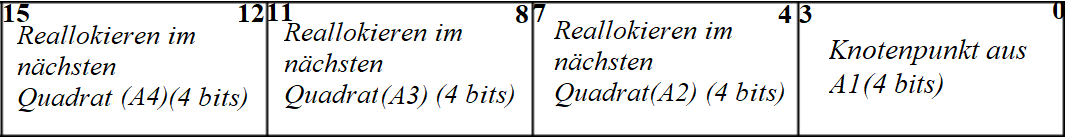
\includegraphics[width=12cm]{Zahlungskodierung.png}
    \caption{}
    \label{fig:Zahlungskodierung.png}
\end{figure}
Wir benutzen die Abbildung \ref{fig:Zahlungskodierung.png}, um die ersten 16 Bits der Iteratorvariable verständlicher zu machen. Das erste Nibble (Bits 0 bis 3) entspricht dem Knotenpunkt aus $A_1$, des reallokiert werden soll. Das passiert durch eine Bijektion, die die Zahl aus dem Nibble nimmt und auf die entsprechende Reihenfolge der Koordinaten als Knotenpunkte von $A_1$ abbildet: \texttt{0000$_2$ $\to$ (0,0),  0001$_2$ $\to$ (0,1),  0010$_2$ $\to$ (0,2),  0011$_2$ $\to$ (1,2),  0100$_2$ $\to$ (2,2),  0101$_2$ $\to$ (2,1),  0110$_2$ $\to$ (1,1),  0111$_2$\newline $\to$ (1,0),  1000$_2$ $\to$ (2,0)} . Z.B. wenn die ersten vier Bits \texttt{0100$_2$} sind, heißt, dass (2,2) Knotenpunkt zur entsprechenden $An_$ Kurve reallokiert sein sollte. Die restlichen Bits der Iteratorvariable bilden eine Kette aus Nibbles (obige Abbildung). Jeder dieser Nibbles setzt der entsprechende Knotenpunkt von $A_1$ aus dem ersten Nibble auf dem Quadrat $Q_i$ ($i \in \{0,1,2,3,4,5,6,7,8\}$) in der nächsten Kurve um. Mit dieser Umsetzung werden die Regeln des entsprechenden Quadrats gehalten. Da die Struktur der Peano-Meander -Kurve eindeutig ist, gelten dieselbe Regel der Quadrate von $A_2$ auch für $A_n$. Der einzige Unterschied ist der Offset. Z.B. \texttt{(0101 1000 0010 0100)}$_2$ sagt uns folgendes:
\begin{enumerate}
  \item nehme (2,2) Koordinatenspunkt (erster Nibble).
  \item stelle ihn erstens im $A_2$ im Quadrat 2(zweiter Nibble). Halte die Regeln von Q2.
  \item stelle der modifizierten Koordinatenpunkt im $A_3$ im Quadrat 8(dritter Nibble). Halte die Regeln von Q8 für der neu modifizierte Koordinatenpunkt aus 2).
  \item und letztlich stelle ihn im $A_4$ im Quadrat 5(vierter Nibble). Halte die Regeln von Q5 für der neu modifizierte Koordinatenpunkt aus 3)
\end{enumerate}
Was nur jetzt fehlt, ist die Offsets für beliebiges $n$  einzutragen.\newline

\large\textbf{Offsets für beliebiges n berechnen}\newline

Offensichtlich ist der Offset $(x,y) \to (x+k_1,y+k_2)$ für beliebiges $n$ nicht $k_1\,_,_2\in\{0,3,6\}$, da für $n>2$ die neun Quadraten größer als $3\times3$ sind. Die Anzahl der Koordinatenpunkte von $A_n$ ist $9^n=3^{2 \cdot n}$. Um die Berechnung iterativ durchzuführen, beginnen wir mit einer Länge $l=3$ (die Länge einer der Achsen von $A_1$) und multiplizieren $l$ in jede Iteration mit drei $(l=3 \cdot l)$, um die Länge der nächsten Kurve zu berechnen. Da alle neun Quadraten immer identische Größe haben und $l=3^i$ für $A_i$, folgt, dass die Länge jedes Quadrates in $A_i$ gleich $l$'$=l/3=3^i/3=3^{i-1}$ ist. Somit ist der Offset für $A_i$ ist $(x,y) \to (x+k_1,y+k_2)$ für $k_1\,_,_2\ \in \{0, 3^{i-1}, 2 \cdot 3
^{i-1}\}$, wobe $i \in \{1, \dots, n\}$ ist. Schließlich können wir unseren Algorithmus für beliebiges $n$ formulieren:
\begin{enumerate}
  \item Iteriere $9^n$ Mal über die natürlichen Zahlen und überspringe Zahlen, die irgendeinen Nibble größer als 8 haben.
  \item Für jede Iteration nehme erstens die ersten vier Bits der Iteratorvariable - nämlich der entsprechende Knotenpunkt aus $A_1$
  \item Füge eine innere Schleife über $n$ ein, die die Aufgabe hat, auf die anderen Nibbles zu iterieren und den Offset zu inkrementieren. Für jede solche Iteration versetze den Koordinatenpunkt aus 2. in dem entsprechenden Quadrat, indem die oben definierten Regel in den Quadraten von $A_2$ bzw. An gehalten werden sollen.   
\end{enumerate}

\large\textbf{SVG und C}\newline

Wir haben diesen Algorithmus in Assembler implementiert und die Koordinaten als Abfolge der Knotenpunkte der Peano-Meander-Kurve $n$-ten Grades richtig repräsentiert. Um das alles darzustellen, erstellen wir eine SVG-Datei. Es gibt aber ein Problem damit- unser Anfangspunkt (0,0) liegt unten links, was sich bei SVG-Dateien oben links befindet. Wir wollen natürlich dieses Problem lösen, ohne unseren Algorithmus zu wechseln.  Wir haben eine Lösung auch dafür gefunden: wir haben alle Koordiantenpunkte mit $-1$ multipliziert, damit unsere Kurve nicht „gespiegelt“ ist und mit dem entsprechenden Offset und Skalierung hatten wir am Ende unsere Peano-Meander-Kurve n-tes Grades in eine SVG-Datei erfolgreich erzeugt. 

% TODO: Je nach Aufgabenstellung einen der Begriffe wählen
\section{Korrektheit}
\noindent\begin{minipage}{.60\textwidth}
Wie oben erwähnt, ist die Anzahl der Koordinatenpunkte $3^{2n}$ ($n$ ist der gewünschte Grad). Das Programm erhält beim Funktionsaufruf den Grad $n$, wobei  $n \in \{1,2,…,8\}$, und dann wird automatisch alles berechnet, eine SVG Datei erstellt und der Firefox Webbrowser geöffnet, um die Grafik der Kurve anzuzeigen. Im Rahmen der genannten Beschreibung, per Hand und durch mehrere Tests berechnet das Programm genau die richtigen Koordinaten und gibt die zugehörige Grafik aus. Es wurden auch Randfälle betrachtet, da unsere Eingabe beschränkt ist.
Beispiel Für $n = 3$:\newline
\end{minipage}%
\begin{minipage}
    \centering
    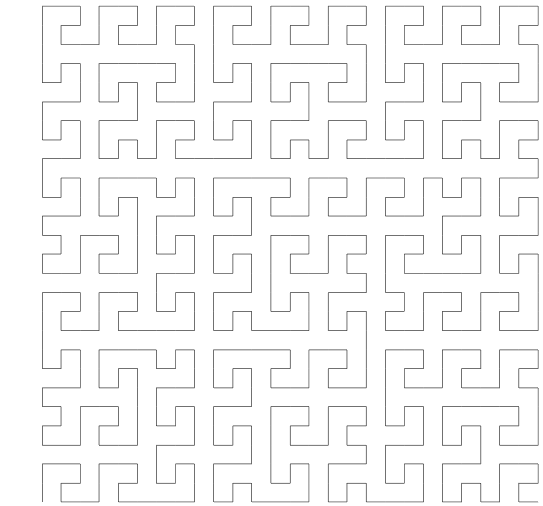
\includegraphics[width=6cm]{N3.PNG}
    %\caption{Peano-Meander-Kurve Grad 3}
    \label{fig:N3.png}
\end{minipage}


\large\textbf{Warum ist die Eingabe beschränkt?}\newline
Die Eingabe wurde auf 8 beschränkt, damit das Programm in sinnvoller Zeit laufen kann. Bei der Eingabe von 9 braucht es ca. 37 Sekunden zur Berechnung der Koordinaten und ca. 20 Minuten beim Schreiben der SVG Datei. Darüber hinaus wirft ein Rechner, dessen 8 GB RAM besetzt ist (nach dem Test), mit Eingabe von 10 einen Segmentation fault-Fehler. Was löste ihn aus? Das Programm bearbeitet 64 Bit Zahlen, und davon zeigen wir den Unterschied zwischen den Graden 9 und 10, wieviel Speicher jeder Grad benötigt. 3ˆ2n ist die Anzahl der Koordinaten und somit müssen wir das Ergebnis mit 2 multiplizieren, um für x und y im Speicher einen Bereich reservieren zu können, also => $2 \cdot 3^{2n}$ 64 Bit Zahlen.
Für $n = 9$ gilt $\frac{2 \cdot 3^{18} \cdot 64\,bit}{8 \cdot 10^9} = 6.198\,GB$ und für $n = 10$ gilt $\frac{2 \cdot 3^{20} \cdot 64\,bit}{(8 \cdot 10^9)} = 55,788\,GB$
Hier können wir leicht den Unterschied zwischen $n = 9$ und $n = 10$ sehen.
Aus den Gründen (Zeit und Speicher) trafen wir die Entscheidung, dass die Eingabe nicht größer als 8 sein darf.\newline

\large\textbf{Was passiert, wenn ein Nutzer eine ungültige Eingabe eingebt?}\newline
Wenn der Nutzer nichts bzw. eine ungültige Eingabe tätigt, erhält er passende Nachricht, die ihm sagt, wie das Programm funktioniert bzw. welche Eingabe eingeben darf. \newline
% einfuegen die helf kumannd

\large\textbf{Anleitung}\newline

Um das Programm ausführen zu können, muss an sich zunächst in dem Verzeichnis /Implementierung/ befinden. In diesem Verzeichnis sollen die folgenden Dateien zur Verfügung stehen:
\begin{itemize}
    \item \textbf{main.c}: für I/O Operationen.
    \item \textbf{peanoM.S}: Implementierung des Algorithmus im Assembler.
    \item \textbf{MakeFile}: Bei der Nutzung der \texttt{make} Befehl kompiliert das Programm automatisch.
    \item \textbf{Peano.sh}: für automatische Öffnung der Grafik in Firefox (nur im Linux funktioniert).
    \item \textbf{Zeitmessung}: Ein Verzeichnis, das alle Dateien enthalten, die für Zeitmessung gehören.     \begin{itemize}
            \item \textbf{main.c, peanoM.S, MakeFile und Peano.sh}: findet man auch in der Zeitmessungs-Verzeichnis. Sie geben die gleiche Funktionalität außer main.c noch an der Konsole ein Zahl ausgibt, die für die gebrauchte Zeit der Berechnung der Koordinaten und des Schreibens der SVG-Datei   
        \end{itemize}
    \item \textbf{Vergleich}: Ein Verzeichnis, wo die in Assembler geschriebene Funktion in C implemintiert ist.
        \begin{itemize}
        \item \textbf{MakeFile}: dient genauso wie in der /Implementierung/ Verzeichnis.
        \item \textbf{peano.h}: die in Assembler geschrieben Funktion wird in C übersetzt
        \item \textbf{cimp.c}: das gleiche wie main.c aber anstatt die peanoM.S zu benutzen, nutzt es die peano.h, um die Koordinaten der Punkten zu berechnen. 
        \end{itemize}
\end{itemize}
Um das Programm zu starten, muss man bei terminal im Verzeichnis /Implementierung/ sein und die folgenden Befehle ausführen:
 \begin{verbatim}
username:~\$ <Path zum Verzeichnis> make
username:~\$ <Path zum Verzeichnis> ./main <gewünschter Grad (n)>
    \end{verbatim}
Nach dem Kompilieren (\texttt{make}) wird eine neue Datei „main“ erstellt, die in der Compile-Zeit erstellt wird. Diese Datei ist ausführbar, daher schreiben wir den zweiten Befehl „\texttt{./main <Grad n>}“, um das Programm auszuführen.

\section{Performanzanalyse}
In diesem Teil analysieren wir unsere Implementierung. Es wird mit einer in C geschriebenen Funktion, die an einer gegebenen Stelle die Koordinaten berechnet, verglichen.\newline
Bevor wir alle Daten zeigen, werden wir uns zuerst über die Hardware informieren, wo der Code getestet wurde. \texttt{CPU: Intel(R) Core (TM) i5-6200U (Single Core), 2.30GHz-2.40GHz, RAM: 8.00GB \System type: 64-bit Betriebssystem, x64-based processor, Betriebssystem: Windows 10 Home (Version 1903), \newline Genutzte Compiler: GCC 7.4.0 mit der Option -O2}\newline

\large\textbf{Analyse der Assemblerteil}\newline

Die Grafik {\footnotesize{(Abbildung} \ref{fig:C-Assembler-Zeit-Grafik.png})} stellt die Laufzeitanalyse für die in Assembler und in C geschriebene Peano-Meander-Funktion dar. Die Laufzeitmessung wurde für jede Eingabe 3 Mal wiederholt und davon den Durchschnitt berechnet. Diese Tests wurden unter idealen Bedingungen durchgeführt; es waren keine Programme im Lauf und zwischen jeweils 2 Tests gab es eine ca. 5 Sek. lange Pufferzeit, das heißt, wir versuchten den Hauptspeicher leer (außer dem Betriebssystem) zu halten und dann nur das Programm laufen zu lassen.
\begin{figure}[htp]
    \centering
    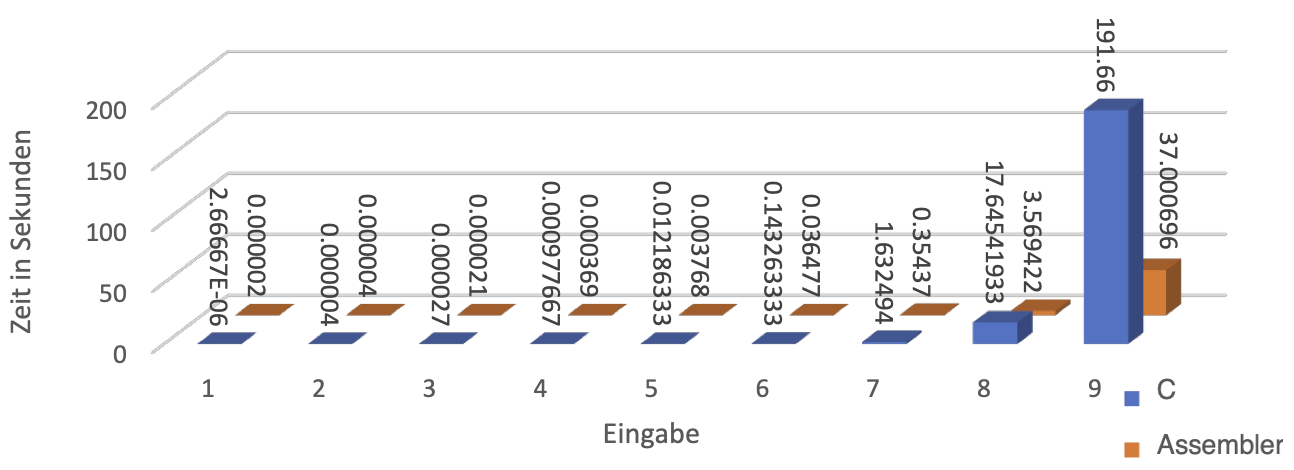
\includegraphics[width=12cm]{C-Assembler-Zeit-Grafik.png}
    \caption{Zeit der Berechnung der Koordinaten von C und Assembler}
    \label{fig:C-Assembler-Zeit-Grafik.png}
\end{figure}
Betrachtet man nun die aufgestellte Grafik, so kann man feststellen, dass die Laufzeiten beider Funktionen ein exponentielles Wachstum haben. Jedoch ist die in Assembler geschriebene Funktion viel schneller als in C. Man kann leicht bemerken, wie die Zeit in C beim Grad 8 und 9 wächst. Beispielsweise bei 8 wächst die Zeit von ca. $3,56s$ bis $17,6s$, d.h die Laufzeit hat zwischen Assembler und C um ca. 490\% zugenommen und beim Grad 9 hat ca. 510\% lange gedauert.\newline
Es lässt sich eine deutliche Tendenz in Richtung Assembler schneller als C erkennen. Warum schneller?
Bekanntermaßen ist die Assemblersprache schneller als C bzw. andere höhere Programmiersprachen, sie hat nämlich einen direkten Zugriff auf die Hardware und kann dann leichter optimiert werden. Beispielsweise hat man in Assembler und in anderen höheren Programmiersprachen Zugriff auf den Stack. Im Vergleich zu höheren Sprachen kann man im Assembler den Stack leicht kontrollieren und bewegen.\newline

\large\textbf{Analyse des SVG Teils}\newline

Nachdem alle Koordinaten im Speicher berechnet wurden und zur Verfügung stehen, schreiben wir sie in die SVG-Datei, um danach die Peano-Meander-Curve als Grafik anzuzeigen. Aus dem Schaubild {\footnotesize{(Abbildung} \ref{fig:SVG-Zeit-Grafik.png})} geht hervor, dass die Zeit wie bei „Analyse der Assemblerteil“ ein exponentielles Wachstum hat. Jedoch ist im Vergleich zum Assemblerteil die Laufzeit viel größer und das Programm somit viel langsamer. Beispielweise braucht der Assembler bei der Eingabe 8 bzw. 9 ca. $3,56s$ bzw. $37s$ und um eine SVG-Datei zu schreiben ca. $115,2s$ bzw. $1246,35s$. Anders gesagt, der Unterschied zwischen der Berechnung und dem Schreiben beim Grad $9$ ca. $20$ Minuten.\newline
\begin{figure}[htp]
    \centering
    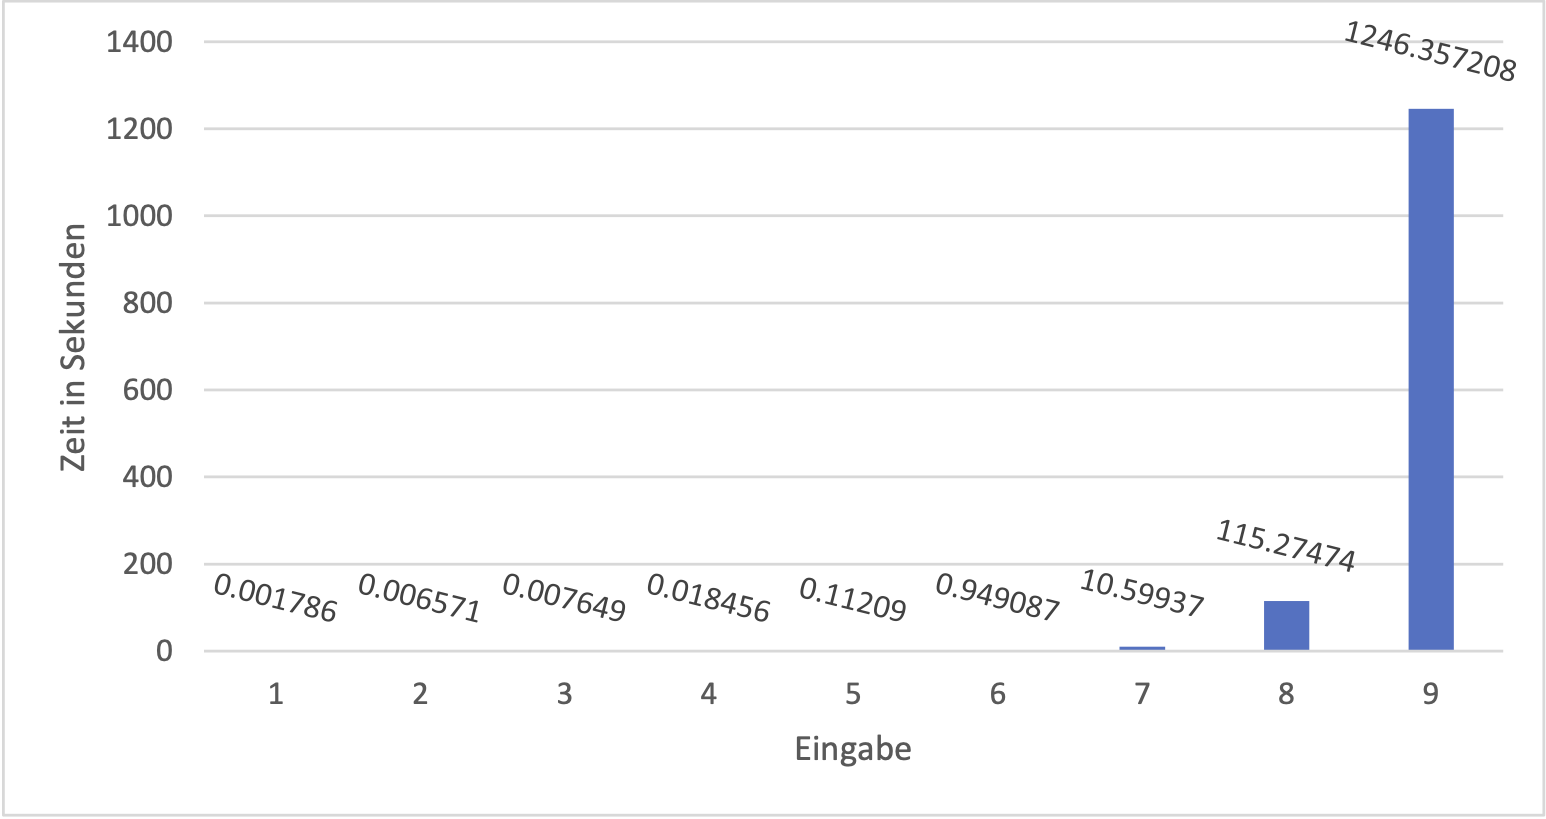
\includegraphics[width=10cm]{SVG-Zeit-Grafik.png}
    \caption{Zeitmessung des Schreibens der SVG-Datei}
    \label{fig:SVG-Zeit-Grafik.png}
\end{figure}
\newline
Darüber hinaus lässt sich noch tiefer mit Hilfe von \texttt{perf} Befehl analysieren. Was ist perf, wie funktioniert es und was gibt es uns von Daten?\newline
\texttt{perf} ist ein Befehl, der während des Programm-Laufes Daten sammelt und sie als ein Datum speichert. Um die Daten zu sammeln, muss man folgendes eingeben: \texttt{perf record -e <Type> ./main <Eingabe>} und zum Zeigen einfach \texttt{perf report} eingeben (Type kann man mit der Eingabe von „\texttt{perf list}“ seinen Wunsch wählen). Nach der cache-misses-Analyse der Funktionen fällt es auf, dass es meistens bei „\texttt{vfprintf} und \texttt{\_IO\_file\_xsputn@@GLIBC\_2.2.5}“ cache misses geschehen.  Für genauere Beschreibung lassen sich die erhaltenden Daten zeigen:\newline
\underline{Mit Assembler:}
 \begin{verbatim}
42.74%  main     libc-2.27.so      [.] vfprintf                       
17.66%  main     libc-2.27.so      [.] _IO_file_xsputn@@GLIBC_2.2.5 
    \end{verbatim}
\underline{C}
\begin{verbatim}
37.43%  cimp     libc-2.27.so      [.] vfprintf                 
31.54%  cimp     libc-2.27.so      [.] _IO_file_xsputn@@GLIBC_2.2.5 
    \end{verbatim}
Erklären lassen sich diese Zahlen möglicherweise mit der Tatsache, dass sowohl im Assembler als auch in C mehr als 60\% von der Cach-misses beim Schreiben der SVG-Datei, d.h bei dem restlichen Programm wurde weniger Cache-misses geschieht
Abschließend kann man feststellen, dass die Laufzeit des Programmes exponentiell wächst.

\section{Zusammenfassung und Ausblick}
In unserem Projekt wurde ein Algorithmus für die Peano-Meander-Kurve entwickelt und implementiert.
Diese Kurven sind ein Teil der Raumfüllung (space filling), die in vielen Bereichen der Informatik, wie z,B Google maps, Image Processing, usw. verwendet wird.\newline
Der Algorithmus wurde in der Assemblersprache implementiert und alle I/O Operationen in C geschrieben. Der Algorithmus berechnet alle Koordinaten unserer Kurve, danach werden alle Koordinaten in eine SVG-Datei geschrieben, um die Kurve mit Firefox zu zeigen. Wie oben in der Korrektheit erwähnt, ist das Programm im Grad zwischen 1 und 8 beschränkt und es wird eine passende Nachricht für eine ungültige Eingabe gezeigt.\newline
Dazu wurde in der Performanceanalyse gezeigt, dass ein Schreiben von SVG-Datei viel Zeit kostet und der größte Anteil der Cache-misses bekommt. Davon gehen wir aus, dass bei der Optimierung vom Schreiben der SVG-Datei wird.

% TODO: Fuegen Sie Ihre Quellen der Datei Ausarbeitung.bib hinzu
% Referenzieren Sie diese dann mit \cite{}.
% Beispiel: CR2 ist ein Register der x86-Architektur~\cite{intel2017man}.
\bibliographystyle{plain}
\bibliography{Ausarbeitung}{}

\end{document}
